\documentclass[10pt,openright,twoside,french]{book}

\usepackage{marvosym}
\input philippe2013
\input philippe2013_activites

\usepackage{docmute}

\pagestyle{empty}

\begin{document}

%___________________________
%===    Page de garde
%------------------------------------------------------

\frontmatter

\titlepage{
\begin{center}
{\Large\bfseries\color{\MaCouleur} Philippe \bsc{De Sousa}}

\vspace*{\stretch{1}}

\begin{tikzpicture}[scale=1.5]
\begin{scope}
% style des noeuds
\tikzstyle{debutfin}=[ellipse,draw,text=red]
\tikzstyle{instruct}=[rectangle,draw,fill=yellow!50]
\tikzstyle{test}=[diamond, aspect=2.5,thick,draw=blue,fill=yellow!50,text=blue]
\tikzstyle{es}=[rectangle,draw,rounded corners=4pt,fill=blue!25]
% style des flèches
\tikzstyle{suite}=[->,>=stealth',thick,rounded corners=4pt]
% placement des noeuds
\node[debutfin] (debut) at (-3,11) {Début};
\node[es] (lire) at (-3,9) {\begin{tabular}{c}Lire un entier positif $A$ \\ Lire un entier positif $B$\end{tabular}};
\node[instruct] (init) at (-3,6) {\begin{tabular}{c}$Q\leftarrow ENT(A \div B)$ \\ $R\leftarrow A - B \times Q$\end{tabular}};
\node[test] (test) at (-3,4) {$R = 0$ \ ?};
\node[es] (affichage) at (-3,1) {$PGCD = B$};
\node[debutfin] (fin) at (-3,-1) {Fin};
\node[es] (remplace) at (1,6) {\begin{tabular}{c}$A\leftarrow B$ \\ $B\leftarrow R$\end{tabular}};
% Placement des flèches
\draw[suite] (debut) -- (lire);
\draw[suite] (lire) -- (init);
\draw[suite] (init) -- (test.north);
\draw[suite] (test) -- (affichage) node[midway,fill=white]{oui};
\draw[suite] (affichage) -- (fin);
\draw[suite] (test) -| (remplace) node[near start,fill=white]{non};
\draw[suite] (remplace) |- (-3,7.5);
\end{scope}
\end{tikzpicture}

\begin{tikzpicture}[remember picture,overlay]
\begin{scope}
\node [rotate=45,scale=10,text opacity=0.2]
at (current page.center) {\color{\MaCouleur} Mathématiques};
\end{scope}
\begin{scope}[xshift=5.5cm,yshift=6cm]
\node [scale=8,color=\MaCouleur] at (0,0) {\seconde};
\node [below=2cm,scale=4,color=\MaCouleur] at (0,0) {Activités};
\end{scope}
\end{tikzpicture}

\vspace*{\stretch{1}}

D'après le programme $\NP{2010}$
\end{center}
} 

\pieddepage{}{}{}
\entete{}{}{}

\mainmatter

\entete{}{{\color{\MaCouleur} \textbullet~\leftmark~\textbullet}}{}
\pieddepage{}{\color{\MaCouleur}$\stackrel{***}{\thepage}$}{}

%------ Chapitre 01 - Equations, inéquations
    %------------------ Activité 1
        \documentclass[10pt,openright,twoside,french]{book}
\input philippe2013
\input philippe2013_activites
\pagestyle{empty}

\begin{document}

\TitreActivite{i.1}{Programme de calcul}

On considère le programme de calcul suivant :\medskip

\psframebox{
\parbox{0.3\linewidth}{
\begin{itemize}
    \item[\textbullet] Choisir un nombre ;
    \item[\textbullet] Retrancher $1$ ;
    \item[\textbullet] \'Elever au carré ;
    \item[\textbullet] Retrancher $12$ ;
    \item[\textbullet] Diviser par $6$.
\end{itemize}
}}\medskip

\begin{enumerate}
    \item Tester ce programme de calcul avec deux nombres différents.
    \item Quelle est la \textit{nature} du résultat obtenu avec $-5$ ?
    \item Quelle est la \textit{nature} du résultat obtenu avec $1$ ?
    \item Quelle est la \textit{nature} du résultat obtenu avec $3$ ?
    \item Quels nombres peut-on choisir pour obtenir le nombre $0$ ?
    \item Recopier la phrase suivante en devinant le dernier mot manquant :
    \begin{center}
    \cursive
    Un programme de calcul est une suite finie d'opérations effectuées dans un ordre précis et appliquées à une donnée de départ (le nombre choisi).\par
    Cela correspond à ce que l'on appelle un a\ldots
    \end{center}
\end{enumerate}


\end{document} \Decouper
    %------------------ Activité 2
        \documentclass[10pt,openright,twoside,french]{book}
\input philippe2013
\input philippe2013_activites

\pagestyle{empty}

\begin{document}

\TitreActivite{i.2}{Motif d'un drapeau}

Une association désire concevoir un drapeau. Pour cela, elle dispose d'une toile carré de côté $8~dm$. Le motif du drapeau est une croix dessinée au centre telle que le montre la figure ci-dessous :

\begin{center}
    \begin{tikzpicture}
        \draw (0,0) -- (4,0) -- (4,4) -- (0,4) -- cycle;
        \draw (0,2.5) -| (1.5,4); \draw (0,1.5) -| (1.5,0);
        \draw (2.5,0) |- (4,1.5); \draw (4,2.5) -| (2.5,4);
        \draw[<->] (0,4.5) -- (4,4.5) node[midway,above] {$8~dm$};
    \end{tikzpicture}
\end{center}

Pour des raisons esthétiques, les concepteurs souhaitent que la croix occupe la moitié de la surface totale du carré. De plus, les espaces vides autour de la croix doivent être des carrés identiques.\medskip

$\rightsquigarrow$ Faire un schéma du drapeau en indiquant toutes les longueurs nécessaires à la conception d'un motif respectant les contraintes énoncées.

\end{document} \clearpage
    %------------------ Activité 3
        \documentclass[10pt,openright,twoside,french]{book}
\input philippe2013
\input philippe2013_activites
\pagestyle{empty}

\begin{document}

\TitreActivite{i.3}{Intervalles de nombres}

Paul a choisi un nombre. Voici quelques indications pour nous aider à le retrouver :
\begin{itemize}
    \item C'est un entier relatif non nul ;
    \item Il est supérieur ou égal à $-5$ ;
    \item Il est strictement inférieur à $4$ ;
    \item C'est un multiple de $3$.
\end{itemize}\bigskip

\begin{enumerate}
    \item Sur une seule droite graduée, représenter les différents indices.
    \item Est-il possible de déterminer le nombre choisi par Paul ?
    \item Parmi tous les indices, modifier un seul mot pour permettre d'avoir une seule solution.
\end{enumerate}
\end{document} \Decouper
        \documentclass[10pt,openright,twoside,french]{book}
\input philippe2013
\input philippe2013_activites
\pagestyle{empty}

\begin{document}

\TitreActivite{i.3}{Intervalles de nombres}

Paul a choisi un nombre. Voici quelques indications pour nous aider à le retrouver :
\begin{itemize}
    \item C'est un entier relatif non nul ;
    \item Il est supérieur ou égal à $-5$ ;
    \item Il est strictement inférieur à $4$ ;
    \item C'est un multiple de $3$.
\end{itemize}\bigskip

\begin{enumerate}
    \item Sur une seule droite graduée, représenter les différents indices.
    \item Est-il possible de déterminer le nombre choisi par Paul ?
    \item Parmi tous les indices, modifier un seul mot pour permettre d'avoir une seule solution.
\end{enumerate}
\end{document} \Decouper
        \documentclass[10pt,openright,twoside,french]{book}
\input philippe2013
\input philippe2013_activites
\pagestyle{empty}

\begin{document}

\TitreActivite{i.3}{Intervalles de nombres}

Paul a choisi un nombre. Voici quelques indications pour nous aider à le retrouver :
\begin{itemize}
    \item C'est un entier relatif non nul ;
    \item Il est supérieur ou égal à $-5$ ;
    \item Il est strictement inférieur à $4$ ;
    \item C'est un multiple de $3$.
\end{itemize}\bigskip

\begin{enumerate}
    \item Sur une seule droite graduée, représenter les différents indices.
    \item Est-il possible de déterminer le nombre choisi par Paul ?
    \item Parmi tous les indices, modifier un seul mot pour permettre d'avoir une seule solution.
\end{enumerate}
\end{document} \clearpage

%------ Chapitre 02 - Coordonnées de points
    %------------------ Activité 1
        \documentclass[10pt,openright,twoside,french]{book}
\input philippe2013
\input philippe2013_activites
\pagestyle{empty}

\begin{document}

\TitreActivite{ii.1}{Calculs de distances\par en utilisant les coordonnées}

La carte ci-dessous représente une partie de la Dordogne dans un repère orthogonal $(O,I,J)$.\par
Les points $B$, $R$ et $S$ représentent respectivement les villes de Beynac, de La Roque-Gageac et de Sarlat.\par
La maison de Paul est situé au niveau du point $P$.\medskip

\begin{center}
    \begin{tikzpicture}[>=latex]
        \draw (0.3,0.25) node[above right] {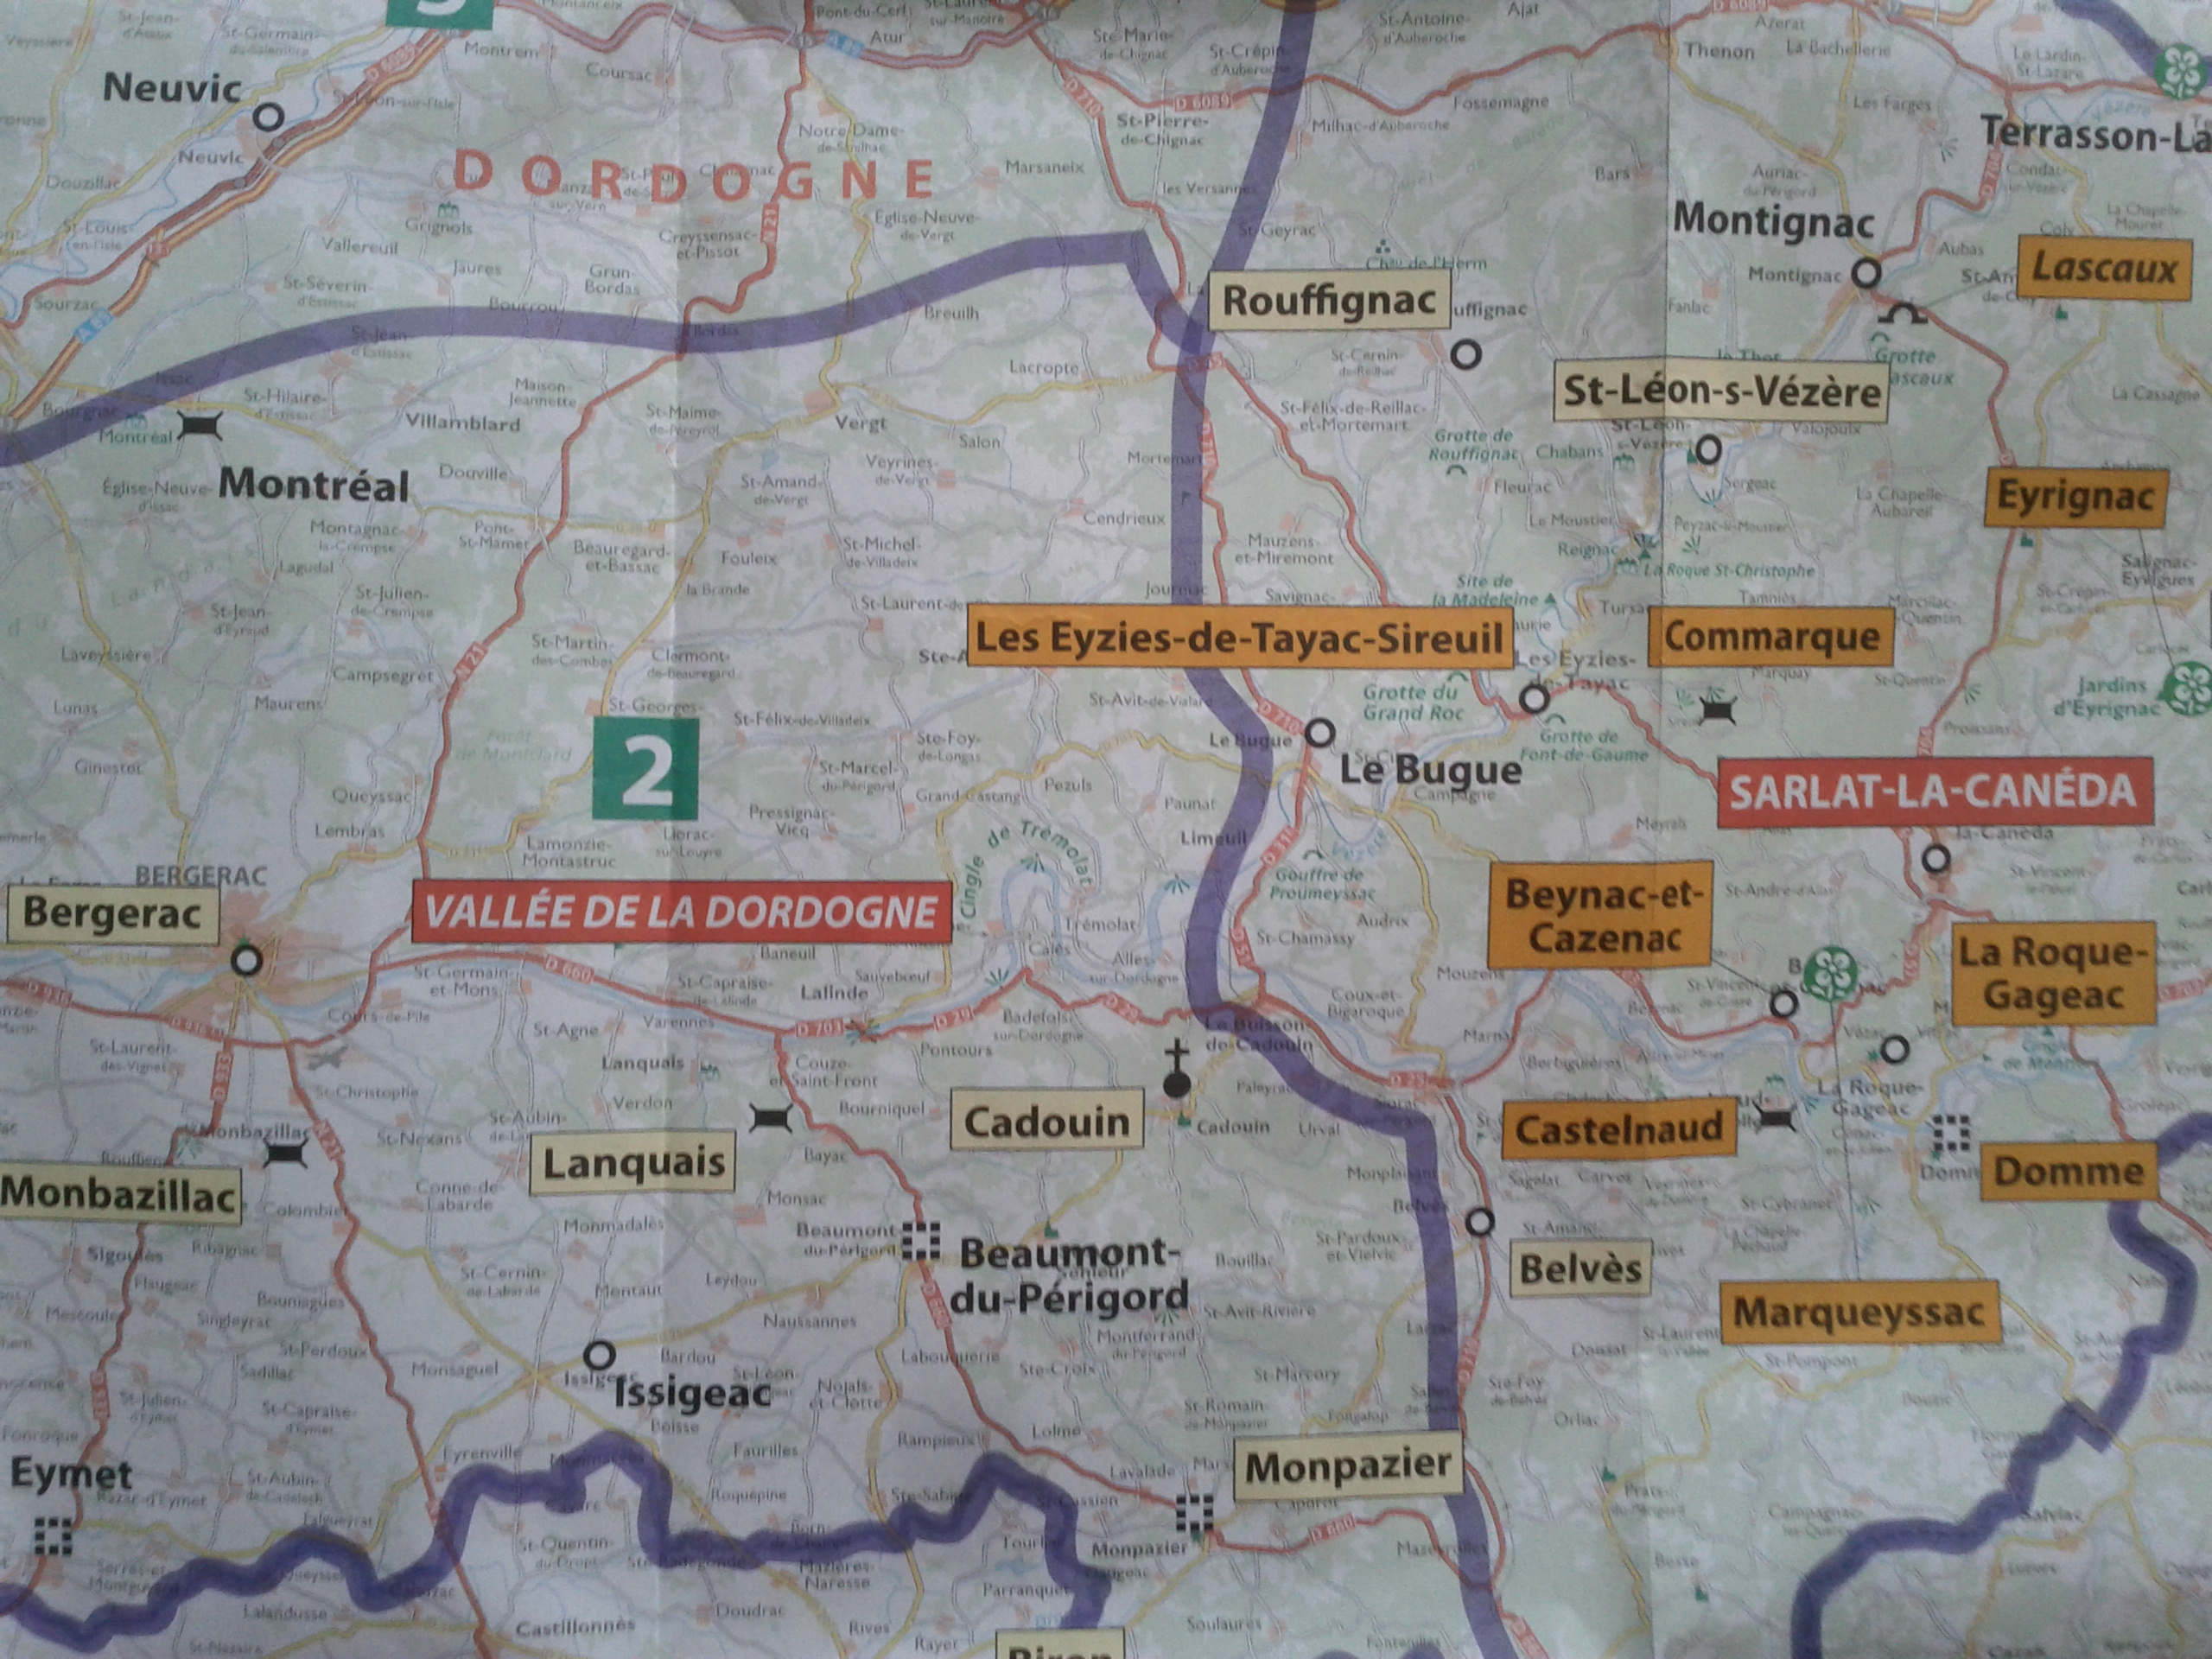
\includegraphics[scale=0.25]{carte_dordogne.ps}};
        \draw[very thin] (0,0) grid[xstep=0.5,ystep=0.5] (12,6.2);
        \coordinate (O) at (0,0); \draw (O) node[below left = -2pt] {$O$};
        \coordinate (I) at (0.5,0); \draw (I) node[below=1pt] {$I$} node {|};
        \coordinate (J) at (0,0.5); \draw (J) node[left] {$J$} node[below=-4pt] {--};
        \draw[thick,->] (-0.2,0) -- (12.4,0); \draw[thick,->] (0,-0.2) -- (0,6.4);
        \draw (5.5,1.5) node[scale=1.25] {$\bullet$} node[below left] {\textbf B};
        \draw (7.5,1.5) node[scale=1.25] {$\bullet$} node[above right] {\textbf P};
        \draw (7.5,1) node[scale=1.25] {$\bullet$} node[above right=-2pt] {\textbf R};
    \draw (8,4) node[scale=1.25] {$\bullet$} node[above left] {\textbf S};
    \end{tikzpicture}
\end{center}\medskip

L'unité de longueur est le carreau. Les distances entre deux villes sont calculées en ligne droite.

\begin{enumerate}
    \item Donner les coordonnées des points $O$ ; $I$ ; $J$ ; $R$ ; $B$ ; $S$ et $P$.
    \item Déterminer la longueur $BP$.
    \item À quelle distance, en ligne droite, la maison de Paul se situe-t-elle de La Roque-Gageac ?
    \item Expliquer pourquoi $BR = \sqrt{BP^2 + RP^2}$.
    \item Calculer alors la distance entre Beynac et La Roque-Gageac.
    \item Un oiseau part de la maison de Paul pour se rendre, en ligne droite, à Sarlat. Quelle est la distance parcourue ?
    \item Sachant que la distance réelle entre Sarlat et Beynac est d'environ $7{,}3~km$, en déduire alors la distance réelle que l'oiseau a parcourue.
\end{enumerate}

\end{document}


\clearpage
\strut
\pieddepage{}{}{}
\entete{}{}{}
\vspace{\stretch{1}}

\[***\]

\begin{center}
\'Ecrit par Philippe \bsc{De Sousa}.\par
Dernière modification le \today.
\end{center}

\end{document} 